\begin{figure}
	\tikzsetnextfilename{riparametrizzazione-superfici}
	\centering
	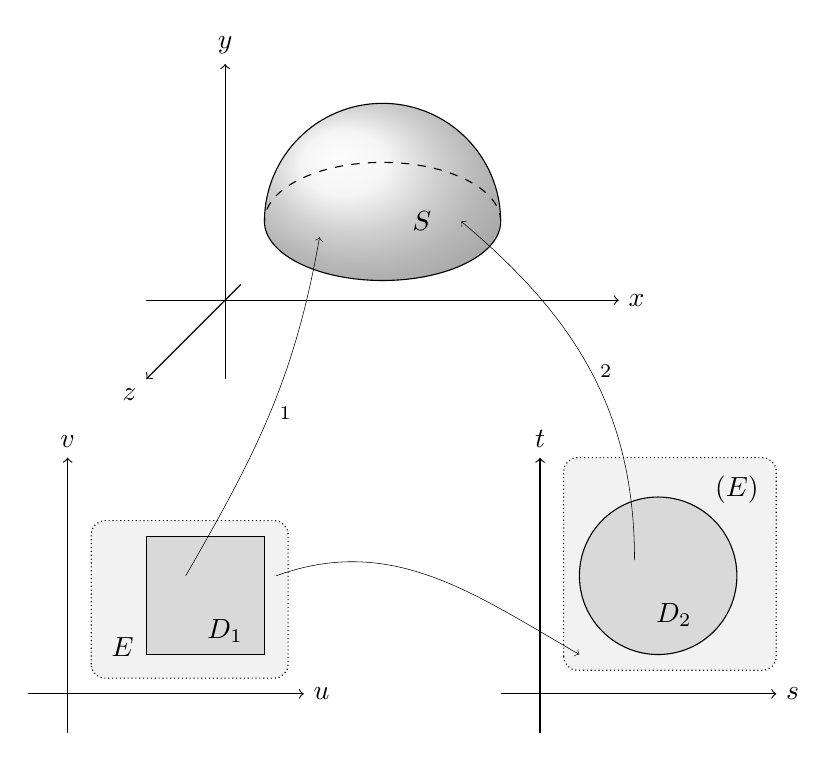
\begin{tikzpicture}
		% Dove possibile ho usato delle coordinate relative alle varie origini dei sistemi di assi
		% che ho disegnato, in modo da facilitare le modifiche.
		% Purtroppo \node e \coordinate ammettono solo coordinate assolute...

		% Piano R^2 per il dominio D_1
		\coordinate (O1) at (0,0);
		\draw [black,->] (O1) +(-.5,0) -- ++(3,0) node[right]{$u$};
		\draw [black,->] (O1) +(0,-.5) -- ++(0,3) node[above]{$v$};

		\draw [fill=black!5!white,densely dotted,rounded corners=5pt] (.3,.2) rectangle +(2.5,2);
		% Disegno un insieme (i.e. E_1) che includa D_1 (il contorno punteggiato dovrebbe
		% suggerire che è un insieme aperto). Dato che va sullo sfondo, lo disegno per primo
		% altrimenti copre D_1.
		\node (E1) at (.7,.6) {$E$};
		\draw [fill=black!15!white,solid] (O1) +(1,.5) rectangle +(2.5,2); % Il dominio D_1
		\node (D1) at (2,.8) {$D_1$};

		% Piano R^2 per il dominio D_2 (traslato di (6,0) rispetto al precedente)
		\coordinate (O2) at (6,0);
		\draw [black,->] (O2) +(-.5,0) -- ++(3,0) node[right]{$s$};
		\draw [black,->] (O2) +(0,-.5) -- ++(0,3) node[above]{$t$};
		
		\draw [fill=black!5!white,densely dotted,rounded corners=5pt] (O2) +(.3,.3) rectangle ++(3,3); % tau(E)
		\node (E2) at (8.5,2.6) {$\vtau(E)$};
		\draw [fill=black!15!white,solid] (O2)+(1.5,1.5) circle (1); % Il dominio D_2
		\node (D2) at (7.7,1) {$D_2$};

		% Spazio R^3 per la superficie (traslato di (2,5) rispetto al piano di D_1)
		\coordinate (O3) at (2,5);
		\draw [black,->] (O3) +(-1,0) -- ++(5,0) node[right]{$x$};
		\draw [black,->] (O3) +(0,-1) -- ++(0,3) node[above]{$y$};
		\draw [black,->] (O3) +(.2,.2) -- ++(-1,-1) node[below left]{$z$};

		\coordinate (C) at (4,6); % Coordinata del centro della "sfera" (relativa a O1)
		\shade[ball color=black!10!white,semitransparent] (C) +(-1.5,0) arc (180:360:1.5 and .75) arc (0:180:1.5);
		% Crea una sfumatura che ricorda la luce riflessa da una sfera (il percorso specificato è il contorno
		% della figura disegnata con i tre archi), come al solito da disegnare prima delle linee di contorno
		\draw[dashed] (C) +(1.5,0) arc (0:180:1.5 and .75); % Semicirconferenza "nascosta" dietro
		\draw (C) +(-1.5,0) arc (180:360:1.5 and .75); % Semicirconferenza "di fronte"
		\draw (C) +(1.5,0) arc (0:180:1.5); % L'arco più grande
		\node (S) at (4.5,6) {$S$};

		% Funzioni tra gli insiemi
		% (Non so bene come usare qui le coordinate relative...)
		\draw [very thin,->] (2.65,1.5) to[out=20,in=150] node[above] {$\vtau$} (6.5,.5);
		\draw [very thin,->] (1.5,1.5) to[out=60,in=260] node[right] {$\vphi_1$} (3.2,5.8);
		\draw [very thin,->] (7.2,1.7) to[out=90,in=320] node[right] {$\vphi_2$} (5,6);
	\end{tikzpicture}
	\caption{Riparametrizzazione di una superficie tramite un diffeomorfismo.}
	\label{fig:riparametrizzazione-superfici}
\end{figure}
